\documentclass{article}
\usepackage{graphicx} % Required for inserting images
\usepackage[utf8]{inputenc}
\usepackage{amsmath}
\usepackage[margin=1in]{geometry}
\usepackage{polyglossia}
\setdefaultlanguage{english}
\setotherlanguage{bengali}
\usepackage{fontspec}
\setmainfont{Times New Roman}
\newfontfamily\bengalifont{Kalpurush}
\newcommand{\textben}[1]{{\bengalifont #1}}

\title{\huge Topical Note on Numerical Method lecture 1}
\author{\textben{ দেবাশীষ চক্রবর্তী} \\
\textben{অধ্যাপক কাজী আশরাফুজ্জামান} \\
MAT-431}
\date{\textben{২২.৫.২০২৫}}
\begin{document}
\maketitle
Numerical Method\textben{ এর বিকল্প নাম হলো} Scientific Computing\textben{।}
\section{Normal Distribution CDF}
Normal Distribution\textben{ এর} PDF \textben{কে} closed form \textben{এ সমাকলন করা যায় না।}
\begin{figure}[htbp]
  \centering
  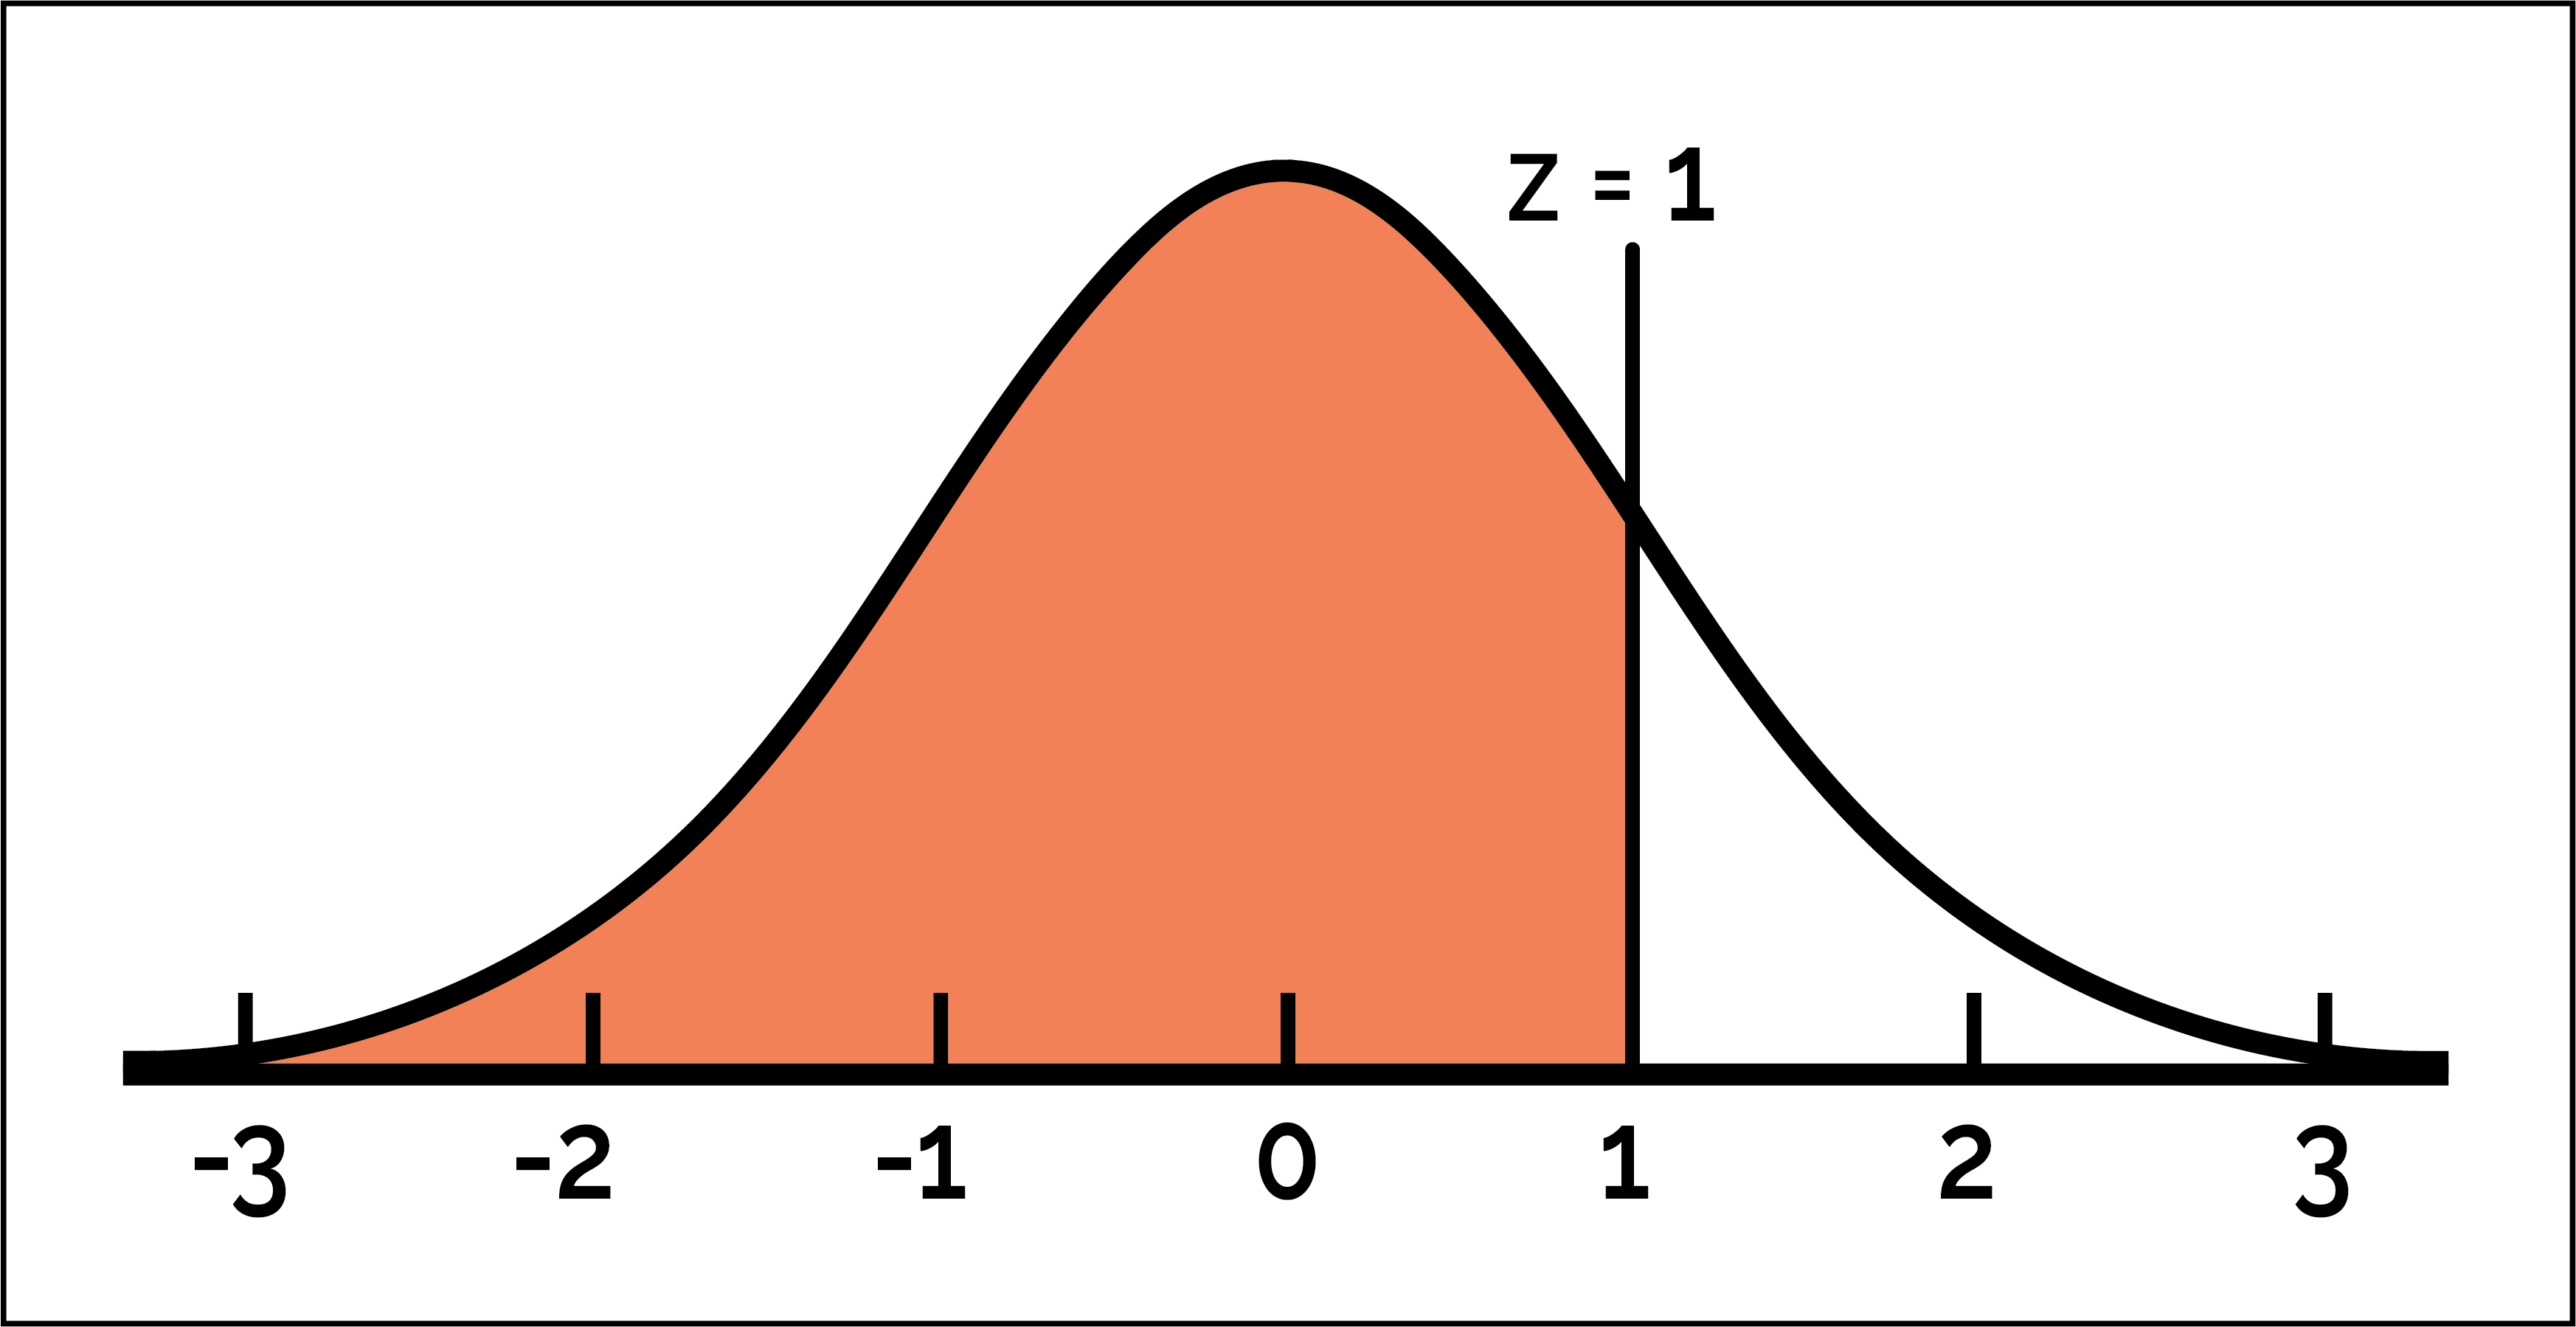
\includegraphics[width=0.6\textwidth]{Normal_Distribution.png}
\end{figure}\\

Normal Distribution CDF, 
$$f_X(x) = \int_{-\infty}^x \frac{1}{\sqrt{2\pi}}e^{-\frac{y^2}{2}}dy$$
\textben{আমরা এই সমাকলনটি বিভিন্ন পদ্ধতিতে গণনা করতে পারি।} \\
\begin{enumerate}
\item \textbf{Riemann Sum:} \textben{একটি} Riemann sum \textben{বক্ররেখার নিচে আয়তক্ষেত্রগুলির ক্ষেত্রফল যোগ করে একটি ফাংশনের নির্দিষ্ট সমাকলনের আনুমানিক মান নির্ণয় করে।}
\item \textbf{Monte Carlo Method:} \textben{সমাকলন গণনার জন্য} Monte Carlo method \textben{এলোমেলো নমুনা সংগ্রহ এবং গড় গণনা ব্যবহার করে একটি নির্দিষ্ট সমাকলনের মানের আনুমানিক মান নির্ণয় করে।}
\item \textbf{Quadratic Equation:} \textben{এলোমেলো ৩টি বিন্দু ব্যবহার করে আমরা একটি দ্বিঘাত সমীকরণ পেতে পারি যা থেকে আমরা আরো নির্ভুলভাবে ক্ষেত্রফল গণনা করতে পারি।}
\end{enumerate}
\textbf{Lab assignment 1:} \textben{এলোমেলো বিন্দু} (Monte-Carlo method) \textben{ব্যবহার করে} Normal Distribution CDF \textben{গণনা করার জন্য একটি প্রোগ্রাম লিখুন।}
\newpage
\section{Modeling}
\textben{নিউমেরিক্যাল মেথডস এর ক্ষেত্রে,} "modeling" \textben{বলতে বোঝায় একটি বাস্তব জগতের ভৌত সিস্টেম বা ঘটনার আচরণ পূর্বাভাস দেওয়ার জন্য একটি গাণিতিক উপস্থাপনা তৈরি করা।}
\begin{itemize}
    \item \textbf{Approximation:} \textben{মডেলিং এ} approximation \textben{বলতে জটিল সিস্টেম বিশ্লেষণের জন্য সরলীকৃত উপস্থাপনা বা কৌশল ব্যবহার করার অনুশীলনকে বোঝায়, যেখানে স্বীকার করা হয় যে মডেলটি বাস্তব জগতের পরিস্থিতির একটি নিখুঁত প্রতিরূপ নয়।}
    \item \textbf{Modeling Errors:}
    \begin{enumerate}
\item Formatting Error
\item Quantization Error
\item Rounding Error
\item Absolute Error
\item Relative Error
\end{enumerate}
    
\end{itemize}
\section{Catastrophic Cancellation:}
\textben{যখন আমরা একটি খুবই বড় সংখ্যা যেমন} Avogadro's number ($6.023 \times 10^{23}$) \textben{থেকে একটি খুবই ছোট সংখ্যা (ইলেকট্রন ভর) বিয়োগ করি, তখন ফলাফল বড় সংখ্যাটিই মনে হয় এবং ছোট সংখ্যাটি সম্পূর্ণভাবে উপেক্ষিত হয়, এই ঘটনাকে} catastrophic cancellation \textben{বলে।}
\section{Floating point sum}
\textben{আমরা ৩টি পদ্ধতি ব্যবহার করে} floating point sum \textben{গণনা করতে পারি।}
\begin{enumerate}
\item Random sum
\item Increasing sum
\item Decreasing sum
\end{enumerate}
\textbf{Lab assignment 2:} \textben{১০০০০টি} floating point \textben{সংখ্যার যোগফল গণনা করার জন্য একটি প্রোগ্রাম লিখুন।}
\section{Linear \& Non-linear equation}
\subsection{Linear Equation:}
$f(x)$ linear \textben{হবে যদি এবং কেবলমাত্র যদি} scalar $a$ \textben{এবং} $b$ \textben{এর সাথে} $x_1$ \textben{এবং} $x_2$ \textben{বিন্দুর জন্য,}
$$f(ax_1 + bx_2) = af(x_1) + bf(x_2)$$
\subsection{Non-Linear Equation:} 
\begin{enumerate}
\item  \textbf{Transcendental equation:} \textben{একটি} transcendental nonlinear equation \textben{হল এমন একটি সমীকরণ যাতে এমন ফাংশন রয়েছে যা} algebraic \textben{নয়, অর্থাৎ সেগুলো বহুপদী সমীকরণের সমাধান হিসেবে প্রকাশ করা যায় না। উদাহরণের মধ্যে রয়েছে ত্রিকোণমিতিক, লগারিদমিক, বা সূচকীয় ফাংশনের সমীকরণ।}
\item \textbf{Algebraic equation:} $f(x) = 0$ \textben{ধরনের একটি সমীকরণ} algebraic \textben{হবে যদি এতে} $x$ \textben{এর ঘাত থাকে, অর্থাৎ,} $f(x)$ \textben{একটি বহুপদী।}
\end{enumerate}
\newpage 
\section{Analytical Question}
\subsection{}
\begin{figure}[htbp]
  \centering
  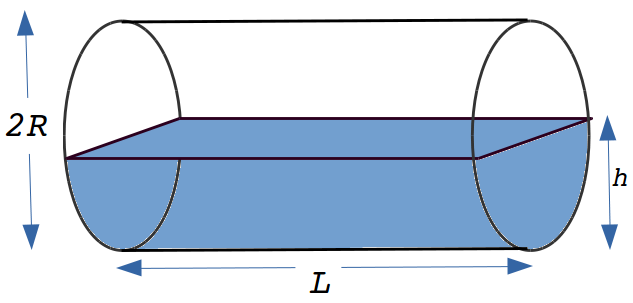
\includegraphics[width=0.6\textwidth]{cylinder.png} % change filename and size as needed
  
  \label{fig:my_label}
\end{figure}
\textben{একটি সিলিন্ডার অনুভূমিক পাশে শুয়ে আছে এবং এটি একটি নল দিয়ে ক্রমাগত পানি দিয়ে পূর্ণ হচ্ছে। সেই সিলিন্ডারের আয়তনের এক-চতুর্থাংশ} ($\frac{1}{4}$) \textben{পূর্ণ করতে মাটি থেকে পানির স্তরের উচ্চতা} ($h$) \textben{কত হবে?}
\subsection{}
\textben{২×২ ম্যাট্রিক্স ব্যবহার করে} fibonacci number recurrence \textben{প্রকাশ করুন।}
\end{document}